% Written with Elsevier's elsarticle LaTeX template (elsarticle.cls),
% the template for the Journal of Financial Economics and other Elsevier journals.
\documentclass[preprint,letterpaper,11pt,authoryear]{elsarticle}
\usepackage{lmodern}
\usepackage[margin=1in]{geometry}
\usepackage{amsmath}
\usepackage{graphicx}
\usepackage{booktabs}
\usepackage{array}
\usepackage[hidelinks]{hyperref}
\hypersetup{pdftitle={What Explains Systolic Blood Pressure in U.S. Adults?},pdfauthor={Nowshed Hossain Imran}}

% Notes printed under a table or figure
\newenvironment{tablenotes}{\par\vspace{3pt}\begin{minipage}{0.95\linewidth}\footnotesize\textit{Note:} }{\end{minipage}}
\newenvironment{figurenotes}{\par\vspace{3pt}\begin{minipage}{0.95\linewidth}\footnotesize\textit{Note:} }{\end{minipage}}

% Footer on the first page
\myfooter[L]{Course project, STAT 5543 Applied Regression Analysis, Oklahoma State University, revised October 2026}

\begin{document}

% let tables share a page with text instead of sitting alone on a float page
\renewcommand{\topfraction}{0.9}
\renewcommand{\textfraction}{0.1}
\renewcommand{\floatpagefraction}{0.8}

\begin{frontmatter}

\title{What Explains Systolic Blood Pressure in U.S. Adults? A Cross-Section Regression Study with NHANES 2011 to 2012}

\author{Nowshed Hossain Imran}
\affiliation{organization={Spears School of Business, Oklahoma State University},
             city={Stillwater},
             state={OK},
             country={USA}}

\begin{abstract}
I use 2,126 fasting adults from NHANES 2011 to 2012 to study how age, gender, race, smoking, diabetes and blood lipids relate to systolic blood pressure. Blood pressure rises with age, and it rises faster for women: at age 50 women are 3.5\% lower than men, but the gap closes at about age 69. Black adults have 5.0\% higher blood pressure than White adults and people with diabetes 3.7\% higher, holding the other factors fixed. The three lipid measures matter together ($p < 0.001$) but their effects are small, and smoking does not matter once the other factors are in the model ($p = 0.27$). Before reading these numbers I checked the conditions a regression needs. The spread of the errors is not constant, so all tests use robust standard errors, and blood pressure medication is left out because it is driven by blood pressure itself. The results stay much the same with other estimation methods.
\end{abstract}

\begin{keyword}
Blood pressure \sep NHANES \sep Cross-section regression \sep Heteroskedasticity
\JEL I12 \sep C21
\end{keyword}

\end{frontmatter}

\section{Question and Main Findings}

High blood pressure is one of the most common health risks in the United States. The course project asked us to build a multiple regression model that explains systolic blood pressure with demographic and clinical variables. My first version did that by searching for the model with the best fit. However, a good fit does not tell what each coefficient means, so in this revision I followed the steps from my econometrics course (Wooldridge 2020): decide what each variable should capture, check whether the regression's conditions hold, fix what fails, and only then read the results. I test two hypotheses.

\begin{itemize}
  \item H1: Holding other factors fixed, blood pressure rises with age, and it rises differently for men and women.
  \item H2: Holding other factors fixed, blood lipids (HDL, LDL and triglycerides) are related to blood pressure.
\end{itemize}

Both are supported. Ten more years of age go with 2.3\% higher blood pressure for a 50-year-old man and 4.3\% for a 50-year-old woman, and this difference between men and women is clearly significant ($p < 0.001$). The three lipids are jointly significant ($p < 0.001$). It is important to note that, these are associations from one point in time. They tell who has higher blood pressure, not what would happen if a person's cholesterol were changed.

\section{Data and Method}

\subsection{Data}
The data come from the National Health and Nutrition Examination Survey (NHANES) of the CDC, in the cleaned form provided by the cardioStatsUSA package (Jaeger, Chen and Muntner). Systolic blood pressure is the average of up to three readings. The 2011 to 2012 cycle has 5,615 adults. LDL cholesterol and triglycerides are measured only for people in the morning fasting group, so 3,213 adults do not have them. Of the 2,187 complete cases, I drop 19 pregnant women and 42 people with triglycerides of 400 mg/dL or more, because NHANES calculates LDL with the Friedewald formula (Friedewald, Levy and Fredrickson 1972) and the formula is not valid above that level. The final sample is 2,126 adults.

\subsection{Model}
Blood pressure has a long right tail (skewness 1.07). Taking the log brings the skewness down to 0.48, and it also means each coefficient can be read as an approximate percentage change. Age enters with a squared term because blood pressure rises slowly in young adults and faster later in life. I center the continuous variables (age at 50, HDL at 50 mg/dL, LDL at 110 mg/dL, both lipids in steps of 10 mg/dL), so the gender coefficient describes a typical person instead of a newborn.

\begin{align}
\log(\text{BP}_i) = \beta_0 &+ \beta_1 \text{Age}_i + \beta_2 \text{Age}_i^2 + \beta_3 \text{Women}_i + \beta_4 (\text{Age}_i \times \text{Women}_i) \nonumber \\
&+ \text{race} + \text{smoking} + \beta_5 \text{Diabetes}_i + \beta_6 \text{HDL}_i + \beta_7 \text{LDL}_i \nonumber \\
&+ \beta_8 (\text{LDL}_i \times \text{Women}_i) + \beta_9 \log(\text{Trig}_i) + u_i
\end{align}

Blood pressure medication is left out on purpose. People take medication because their blood pressure is high, and then the medication lowers it. In other words medication is partly an outcome of the dependent variable, and controlling for such a variable (a bad control) would distort the other coefficients (Wooldridge 2020). Section~\ref{sec:robust} shows what happens when it is included anyway.

\subsection{Should Men and Women Share One Model?}
I used a Chow test (Wooldridge 2020) to decide this. First I fit one model for everyone, and then a model where every slope is allowed to differ between men and women. The single model is clearly rejected. Which slopes are actually different? Only age and LDL are. Once those two interactions are in the model, the other ten add nothing ($p = 0.29$), so the main model keeps only these two.

\begin{table}[!htbp]
\centering\small\setlength{\tabcolsep}{4pt}
\caption{Chow Tests: Do Men and Women Share the Same Slopes?}
\begin{tabular}{lcc}
\toprule
Simpler model compared with the fully separate model & $F$-statistic & $p$-value \\
\midrule
No differences between men and women & 9.50 & $<$ 0.001 \\
Only the age slope differs & 2.76 & 0.002 \\
Age and LDL slopes differ (chosen model) & 1.20 & 0.289 \\
\bottomrule
\end{tabular}
\begin{tablenotes}
The fully separate model lets every slope differ by gender. Each row tests whether the differences left out of the simpler model are all zero. A large $p$-value means nothing important was left out. $n = 2{,}126$.
\end{tablenotes}
\end{table}

\section{Checking the Model}
A linear regression gives reliable answers only when a few conditions hold, and Wooldridge (2020) lists six of them. Table 2 shows how I checked each one.

\begin{table}[!htbp]
\centering\small\setlength{\tabcolsep}{4pt}
\caption{Checks on the Main Model}
\begin{tabular}{>{\raggedright\arraybackslash}p{3.3cm}>{\raggedright\arraybackslash}p{4.0cm}>{\raggedright\arraybackslash}p{5.1cm}}
\toprule
Condition & How I checked & What I found and did \\
\midrule
The model has the right shape & RESET test & $p = 0.34$ with the squared age term, 0.02 without it. Keep the log and the squared term. \\
The sample represents the population & Compare the fasting group with the adults left out & Similar blood pressure (122.8 vs 123.2) and gender mix, but 2.5 years older. Noted as a limitation. \\
No variable repeats another & Variance inflation factors & All between 1.02 and 1.22, so no problem. \\
Nothing important is left out or wrongly put in & Medication; obesity & Medication left out as a bad control. Leaving out obesity changes a few coefficients slightly (Table 3). \\
The spread of the errors is constant & Breusch-Pagan and White tests & Both reject ($p < 0.001$). Use robust standard errors and compare with FGLS. \\
The errors are close to normal & Skewness of the residuals & Mildly skewed, but with 2,126 people the usual tests still work. \\
\bottomrule
\end{tabular}
\end{table}

\subsection{What Leaving Out Obesity Does}
Obesity raises blood pressure and is linked to diabetes and lipids, so leaving it out could bias the other coefficients. BMI is available for 2,088 people, so I can measure this bias directly with the omitted variable bias formula (Wooldridge 2020). The change in a coefficient when obesity is left out equals the effect of obesity on blood pressure ($\hat\gamma$) times how strongly that variable is linked to obesity ($\hat\delta$). Obesity raises blood pressure by 1.4\% ($p = 0.024$). In Table 3 the formula matches the actual change for every variable. The diabetes, triglyceride and Black coefficients are slightly too large without obesity, because obese people are more likely to have those characteristics, while HDL is slightly too small. All these biases are small, so I keep obesity out of the main model and keep the full sample.

\begin{table}[!htbp]
\centering\small\setlength{\tabcolsep}{4pt}
\caption{The Bias from Leaving Out Obesity}
\begin{tabular}{lcccc}
\toprule
Variable & Without obesity & With obesity & $\hat\delta$ & Bias $= \hat\gamma\hat\delta$ \\
\midrule
Diabetes & 0.0369 & 0.0341 & 0.206 & $+$0.0028 \\
log(Triglycerides) & 0.0273 & 0.0257 & 0.116 & $+$0.0016 \\
HDL (per 10 mg/dL) & 0.0051 & 0.0061 & $-$0.074 & $-$0.0010 \\
Black & 0.0509 & 0.0489 & 0.145 & $+$0.0020 \\
\bottomrule
\end{tabular}
\begin{tablenotes}
$n = 2{,}088$ adults with BMI. Obese means BMI of 30 or more (36.2\% of the sample). $\hat\gamma = 0.0137$. The first column minus the second equals the bias column.
\end{tablenotes}
\end{table}

\subsection{Unequal Spread of the Errors}
Both tests say the spread of the errors is not the same for everyone (heteroskedasticity), even though it is hard to see in panel (a) of Figure 1. This does not bias the coefficients, but it makes the usual standard errors wrong. There are two common fixes (Wooldridge 2020). Robust standard errors keep the same coefficients and correct the standard errors; here they differ from the usual ones by a factor of 0.92 to 1.14. FGLS instead estimates how the spread changes across people and gives less weight to the noisier observations. FGLS gives almost the same results (Table 5), therefore I report the regular estimates with robust standard errors and use FGLS as a check.

\subsection{Unusual Observations}
One reading is far from what the model predicts (largest studentized residual 4.57). However, no single person moves the results much: the largest Cook's distance is 0.016, far below the usual warning level of 1. Removing the 20 most influential people changes little, and median regression, which is less sensitive to extreme values, tells the same story (Table 5).

\section{Results}
Table 4 gives the main model. Since the dependent variable is in logs, each coefficient is turned into a percentage effect with $100(e^{\beta}-1)$.

\begin{table}[!htbp]
\centering\small\setlength{\tabcolsep}{4pt}
\caption{Main Model: Log Systolic Blood Pressure}
\begin{tabular}{lccc}
\toprule
Variable & \% effect & Robust SE (log points) & $p$-value \\
\midrule
Age, per 10 years (man at 50) & 2.31 & 0.23 & $<$ 0.001 \\
Age squared & & & $<$ 0.001 \\
Women (at age 50, LDL 110) & $-$3.52 & 0.58 & $<$ 0.001 \\
Age $\times$ Women, per 10 years & 1.93 & & $<$ 0.001 \\
Hispanic & $-$0.48 & & 0.512 \\
Asian & $-$0.59 & & 0.429 \\
Black & 5.02 & 0.71 & $<$ 0.001 \\
Other race & 1.10 & & 0.556 \\
Current smoker & 1.14 & & 0.105 \\
Former smoker & 0.34 & & 0.620 \\
Diabetes & 3.75 & 0.89 & $<$ 0.001 \\
HDL, per 10 mg/dL & 0.51 & & 0.020 \\
LDL, per 10 mg/dL (men) & 0.48 & & $<$ 0.001 \\
LDL $\times$ Women & $-$0.60 & & $<$ 0.001 \\
log(Triglycerides) & 2.70 & & $<$ 0.001 \\
\midrule
$R^2$ / adjusted $R^2$ & \multicolumn{3}{c}{0.276 / 0.271} \\
\bottomrule
\end{tabular}
\begin{tablenotes}
OLS, $n = 2{,}126$. Reference groups: men, Non-Hispanic White, never smoked. Robust (HC1) standard errors. The triglyceride coefficient is an elasticity: 10\% higher triglycerides go with 0.25\% higher blood pressure.
\end{tablenotes}
\end{table}

\subsection{H1: Age and Gender}
Because of the squared term, the effect of age grows with age. For men it is 1.7\% per ten years at age 40 and 3.0\% at age 60. For women it is 3.6\% at 40 and 4.9\% at 60. Women start lower, but their faster rise closes the gap at about age 69, after that women are predicted slightly higher (panel (b) of Figure 1). The difference between the male and female age slopes is significant ($p < 0.001$), so H1 is supported.

\subsection{H2: Blood Lipids}
The three lipids are jointly significant (robust $F$-test, $p < 0.001$). Higher triglycerides and higher LDL go with higher blood pressure among men. For women the LDL slope is close to zero ($-$0.12\% per 10 mg/dL, $p = 0.30$), which is the gender difference the Chow test picked up. HDL came out positive, the opposite of what I expected. One possible reason is drinking, which raises both HDL and blood pressure and is not in the model. H2 is supported, but the lipid effects are small next to age, race and diabetes.

\subsection{Other Factors}
Race matters jointly ($p < 0.001$), mainly because of the 5.0\% higher blood pressure of Black adults. Diabetes goes with 3.7\% higher blood pressure. Smoking is not significant, alone or together ($p = 0.27$).

\section{Robustness}
\label{sec:robust}
Table 5 repeats the key estimates with other choices. The main conclusions do not depend on the method. The medication column shows why it is a bad control: adding medication cuts the diabetes effect from 3.75\% to 3.10\%, because people with diabetes are more often treated, while among adults who take no medication the diabetes effect is 4.73\%.

\begin{table}[!htbp]
\centering\small\setlength{\tabcolsep}{6pt}
\caption{Key Effects (\%) with Other Choices}
{\begin{tabular}{lcccc}
\toprule
 & Main & + Medication & FGLS & Median regression \\
\midrule
Age, man at 50 & 2.31 & 1.88 & 2.26 & 2.17 \\
Women & $-$3.52 & $-$3.67 & $-$3.51 & $-$3.92 \\
Black & 5.02 & 4.41 & 4.87 & 4.14 \\
Diabetes & 3.75 & 3.10 & 3.50 & 2.86 \\
HDL, per 10 & 0.51 & 0.55 & 0.39 & 0.41 \\
LDL, per 10 (men) & 0.48 & 0.56 & 0.42 & 0.23 \\
log(Triglycerides) & 2.70 & 2.44 & 3.02 & 2.25 \\
\bottomrule
\end{tabular}}
\begin{tablenotes}
$n = 2{,}126$ in every column. + Medication: blood pressure medication added to the model (its own effect is 4.16\%). Median regression uses bootstrap standard errors; in it the HDL and LDL effects are only marginal ($p = 0.055$ and 0.064), and all others are significant.
\end{tablenotes}
\end{table}

\begin{figure}[!htbp]
\centering
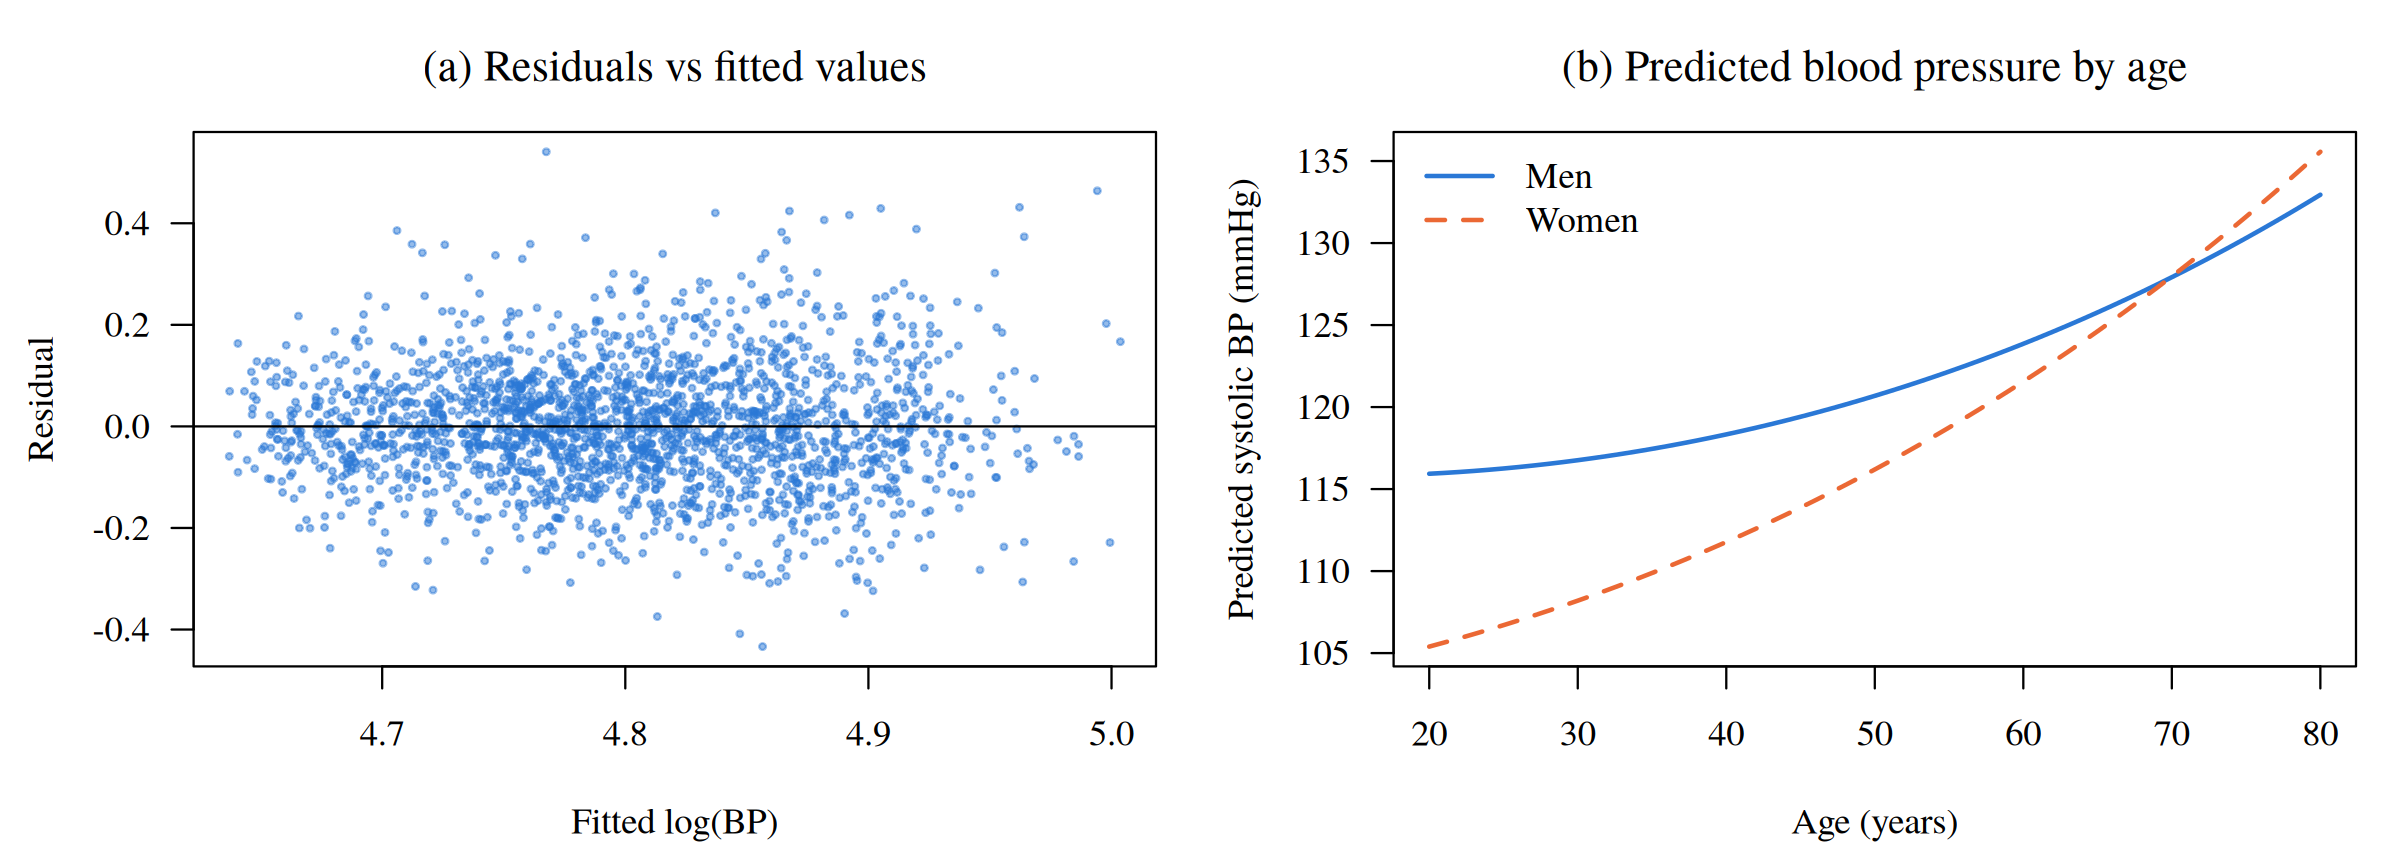
\includegraphics[width=\linewidth]{figure1.png}
\caption{Residuals and Predicted Blood Pressure by Age}
\begin{figurenotes}
Panel (a): residuals against fitted values from the main model. Panel (b): predicted systolic blood pressure by age for men and women, other variables at their reference or centered values.
\end{figurenotes}
\end{figure}

\section{Limitations}
\begin{itemize}
  \item The data are from one point in time, so the estimates are associations. Causality can run the other way for lipids and diabetes, as it does for medication.
  \item The NHANES survey weights are not used, so the estimates describe this sample and are not national averages.
  \item Diabetes and smoking are self-reported. Errors in such variables usually push their coefficients toward zero.
  \item Factors such as obesity, salt intake, alcohol and physical activity are not in the main model. Obesity was checked directly, the others could not be.
  \item Blood pressure is measured on a single day, so day-to-day variation adds noise.
\end{itemize}

\section{Conclusion}
The first version of this project looked for the best fit. Following the econometric steps changed the model in three ways: medication was dropped as a bad control, the gender differences were chosen by a Chow test rather than by search, and the tests moved to robust standard errors after the spread of the errors turned out to be unequal. The results are clear and stable. Blood pressure rises with age and faster for women, it is higher for Black adults and for people with diabetes, and lipids matter together but only a little. A next step would be to use the survey weights and several NHANES cycles, to see whether these patterns hold for the whole population and over time. A good fit is easy to find, knowing what the coefficients mean takes more work.

\begin{thebibliography}{00}
\bibitem[Friedewald et al.(1972)]{friedewald} Friedewald, William T., Robert I. Levy, and Donald S. Fredrickson. 1972. ``Estimation of the Concentration of Low-Density Lipoprotein Cholesterol in Plasma, without Use of the Preparative Ultracentrifuge.'' \textit{Clinical Chemistry} 18 (6): 499 to 502.
\bibitem[Jaeger et al.(n.d.)]{jaeger} Jaeger, Byron C., Ligong Chen, and Paul Muntner. \textit{cardioStatsUSA: Cardiovascular Statistics for the US Population}. R package. NHANES data from the CDC National Center for Health Statistics.
\bibitem[Wooldridge(2020)]{wooldridge} Wooldridge, Jeffrey M. 2020. \textit{Introductory Econometrics: A Modern Approach}. 7th ed. Boston: Cengage.
\end{thebibliography}

\vspace{6pt}
\noindent Code: \href{https://github.com/nowshed-imran/STAT-5543-Project}{github.com/nowshed-imran/STAT-5543-Project}

\end{document}
